\section{Evaluation}
\label{sec:eval}

Evaluation of a construction method like this one is awkward, because the thing to be
evaluated is not a single model's output but a discipline. We report five kinds of
measurement: the graph's scale and internal integrity, the distribution of epistemic
types, precision against an external reference set, the outcomes of adversarial
gates, and one downstream question-answering benchmark. We then state at length what
none of these establish.

\begin{figure}[tbp]
\centering
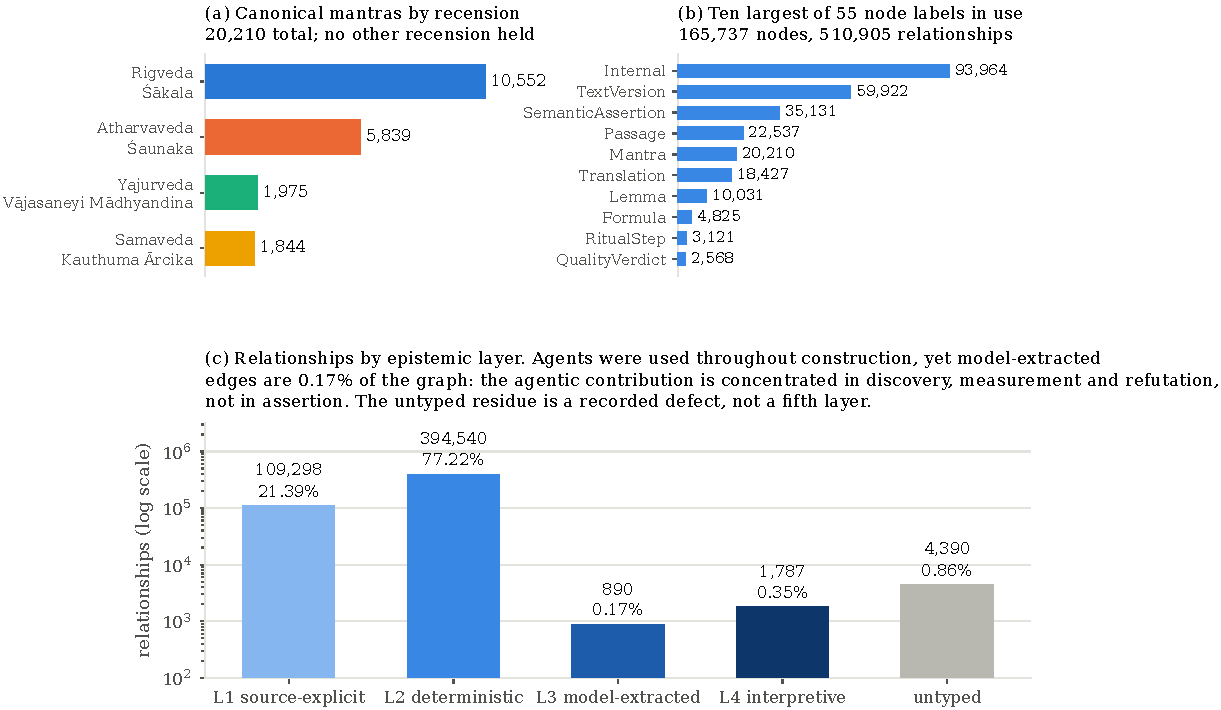
\includegraphics[width=\linewidth]{figures/fig_corpus_and_epistemic.pdf}
\caption{Corpus, graph scale, and the distribution of epistemic types.
\textbf{(a)} The canonical corpus is four named recensions, not ``the Vedas''.
\textbf{(b)} The ten largest node labels; \code{Internal} is a marker on non-public
objects, not a domain type. \textbf{(c)} The paper's central measurement, on a log
scale: agents were used continuously throughout construction, and model-extracted
relationships are 0.17\,\% of the graph. The untyped residue is a recorded defect in
the grading contract, not a fifth layer. Measured on the live store at commit
\code{6bf220c}.}
\label{fig:corpus-epistemic}
\end{figure}

\subsection{Scale and integrity}

% generated by figures-src/make_tables.py -- do not edit
\begin{table}[tb]
\centering
\caption{The fourteen largest node labels and relationship types, of 55 labels
in use and 81 relationship types.
A further label, \code{SourceArtifact}, is declared in the store's token table but
carries no nodes.}
\label{tab:labels}
\small
\begin{tabular}{@{}lr@{\hskip 2em}lr@{}}
\toprule
Node label & Nodes & Relationship type & Edges \\
\midrule
\code{Internal} & 93{,}964 & \code{MENTIONS\_LEMMA} & 154{,}261 \\
\code{TextVersion} & 59{,}922 & \code{HAS\_TEXT\_VERSION} & 59{,}922 \\
\code{SemanticAssertion} & 35{,}131 & \code{HAS\_SEMANTIC\_ASSERTION} & 35{,}131 \\
\code{Passage} & 22{,}537 & \code{ASSERTION\_PREDICATE} & 32{,}938 \\
\code{Mantra} & 20{,}210 & \code{MENTIONS\_ENTITY} & 28{,}122 \\
\code{Translation} & 18{,}427 & \code{ABOUT\_CONCEPT} & 24{,}861 \\
\code{Lemma} & 10{,}031 & \code{USES\_FORMULA} & 22{,}686 \\
\code{Formula} & 4{,}825 & \code{CONTAINS} & 22{,}537 \\
\code{RitualStep} & 3{,}121 & \code{HAS\_TRANSLATION} & 18{,}427 \\
\code{QualityVerdict} & 2{,}568 & \code{HAS\_RISHI} & 17{,}889 \\
\code{RoleFiller} & 2{,}052 & \code{MENTIONS\_DEVATA} & 17{,}165 \\
\code{DerivedMetric} & 1{,}485 & \code{HAS\_CHANDAS} & 16{,}298 \\
\code{PadaParallelGroup} & 1{,}434 & \code{HAS\_DEVATA} & 10{,}558 \\
\code{QAIssue} & 915 & \code{SHARES\_FORMULA\_WITH} & 6{,}148 \\
\bottomrule
\end{tabular}
\end{table}


At the frozen commit the graph holds 165{,}737 nodes and 510{,}905 relationships
across 55 node labels in use and 81 relationship types
(\cref{fig:corpus-epistemic}, \cref{tab:labels}). Of the nodes, 71{,}773 are public
and 93{,}964 carry the internal marker. Every one of the 71{,}773 public nodes has a
non-null public identifier and the identifiers are distinct.

Integrity is gated rather than asserted, and we ran the gates rather than quoting
the project's certification of them. That distinction turned out to matter.

The eleven scorecard gates all read zero: internal leakage, ungraded edges, nodes
without a label, orphan entities, signature violations, undeclared relationship
types, interpretive claims graded other than the weakest tier, claims and metrics
pointing at passages, orphan public nodes, and labels falsely declared unpopulated.

\textbf{The twenty live invariants do not all pass.} Running the suite at the frozen
commit gives 17 ok, 1 warning and \emph{2 failures}:

\begin{center}\small
\begin{tabular}{@{}llr@{}}
\toprule
Severity & Invariant & Edges \\
\midrule
\textsc{fail} & \code{edges\_without\_grade\_basis} & 165{,}788 \\
\textsc{fail} & \code{edges\_without\_attribution\_precision} & 19{,}598 \\
\textsc{warn} & \code{assertions\_without\_predicate\_edge} & 2{,}193 \\
\bottomrule
\end{tabular}
\end{center}

\noindent So 32.5\,\% of edges cannot say \emph{why} they carry the grade they
carry, and 3.8\,\% do not say whether they are a per-verse claim, an inherited
label, a textual mention, or not an attribution at all. Both invariants are declared
at failing severity by the repository itself.

We report this prominently because of how we came to it. An earlier draft of this
paper asserted that all twenty invariants passed, on the authority of the project's
release certification --- which recorded that state truthfully at an earlier census.
We had not run the suite. An adversarial reviewer of this manuscript ran it in one
command and the claim fell. That is precisely the failure the paper is about: a
report was trusted where a measurement was available, by the authors of a paper
arguing that reports are not evidence. It is recorded in
\code{supplementary/peer\_review.md} and we have not smoothed it away here.

What does hold as a universal quantifier, verified: no edge without a quality tier
(510{,}905 of 510{,}905), no unlabelled node, no product node reaching a diagnostic
node, no attribution-precision value outside the declared enumeration, no work
without a scope statement, and no predicate carrying more than one run identifier.

\paragraph{One coverage gap we report rather than round away.} The quality tier is
present on 100.00\,\% of edges. The \emph{knowledge layer} is present on 99.14\,\%:
4{,}390 edges carry no layer, and they are not scattered --- they are 4{,}079
\code{HAS\_PARALLEL\_PADA} edges and 311 \code{REUSES\_TEXT\_FROM} edges. Worse than
their number is the grade they carry: \emph{all 4{,}390 are \code{TIER\_B}}, the tier
the model defines as ``a reproducible rule derived it''. An edge whose origin the
graph does not record is therefore presented to a reader as reproducibly derived.
The tier-from-layer mapping is also not the total bijection \cref{sec:model}
describes: besides the documented candidate rule (292 model-extracted edges at
\code{TIER\_D}), 2{,}469 deterministically derived edges carry \code{TIER\_D} and 36
source-explicit edges carry \code{TIER\_B}. This is a real residual defect in the
graph-wide typing contract, not a fifth layer, and the
percentages in \cref{tab:layers} are computed over all 510{,}905 edges rather than
over the typed subset, so the gap is visible rather than divided away.

\subsection{The distribution of epistemic types}
\label{sec:eval-distribution}

The central measurement of this paper is \cref{tab:layers}. Model-extracted
relationships number 890, or 0.17\,\% of the graph; interpretive claims number
1{,}787, or 0.35\,\%. The remaining 98.6\,\% is either what a source states
(21.39\,\%) or what a reproducible rule derives from what a source states
(77.22\,\%).

\paragraph{The ratio depends on the population, so we give four.} A reviewer of
this manuscript observed, correctly, that 0.17\,\% is the smallest of several
defensible figures and that quoting only it overstates the result. The denominator
of 510{,}905 includes populations no extraction method could ever author ---
154{,}261 lemma mentions, 59{,}922 text-version links, 22{,}537 containment edges
and 18{,}427 translation links, 255{,}147 in all. Over the 255{,}758 edges that
remain once that plumbing is removed, the model-extracted share is 0.35\,\%. Over
the semantic
assertion layer alone --- the population where a model is actually the proposing
mechanism --- it is 2{,}459 of 35{,}131, or \textbf{7.0\,\%}. And if one counts
every edge whose existence is owed to a model proposal rather than only those
carrying the layer, the figure is higher again.

All four are true of different questions. The one the paper's argument needs is not
the smallest but the one over the population at risk: \textbf{where a model could
assert, it authored 7.0\,\% of the assertions, and none of them was promoted}. We
keep 0.17\,\% as the graph-wide figure because a consumer filtering the whole store
is filtering the whole store, and we state the others here so that the choice of
denominator is the reader's rather than ours.

At node level the same shape holds: of 165{,}737 nodes, 2{,}459 carry the
model-extracted layer, all of them \code{SemanticAssertion} nodes with derivation
\code{MODEL\_EXTRACTION}. The remaining 32{,}672 semantic assertions are derived by
morphological rule over a published scholarly annotation or from a treebank
dependency relation, and the project's own code refuses to blend the two totals,
on the ground that a blended figure states a confidence about all 35{,}131
assertions that is true of neither population.

\paragraph{And 89\,\% of the model layer is not wired.} Of the 2{,}459
model-extracted assertions, \textbf{2{,}193 carry no \code{ASSERTION\_PREDICATE}
edge at all} --- their predicate is a property but not a relationship, so
predicate-level traversal cannot see them. The repository's own invariant suite
reports this at warning severity, and it is the third adversarial finding from an
earlier round that was never remediated. It bears directly on the figure above: had
those assertions been wired as the deterministic derivations are, the
model-extracted edge count would be 890 plus 2{,}193, and the graph-wide share
would be roughly 0.6\,\% rather than 0.17\,\%. Part of what the headline ratio
measures is a wiring defect rather than a discipline.

Two further measurements characterise how much the semantic layer withholds. Of the
35{,}131 assertions, 28{,}734 carry \code{roles\_withheld}, and only 341 are
three-slot complete --- that is, fewer than 1\,\% of the semantic assertions assert a
full agent--predicate--patient frame. The layer is overwhelmingly a predicate layer
with the role slots deliberately empty (\cref{sec:failure}, F2).

\begin{figure}[tbp]
\centering
\resizebox{0.95\textwidth}{!}{% GENERATED by figures-src/fig_indra.py -- do not edit by hand.
% Queried live; selection criteria are in that script's docstring.
\begin{tikzpicture}[
  font=\footnotesize, every node/.style={align=center},
  hub/.style={draw=black!65, line width=0.8pt, rounded corners=3pt,
              fill=black!5, inner sep=6pt, font=\bfseries},
  nd/.style={draw=black!40, rounded corners=2pt, inner sep=3pt,
             font=\scriptsize, fill=white, line width=0.4pt},
  l1/.style={nd, fill=SkyBlue!22, draw=SkyBlue!70!black},
  l2/.style={nd, fill=SkyBlue!10, draw=SkyBlue!45!black},
  l3/.style={nd, fill=RoyalBlue!30, draw=RoyalBlue!75!black},
  l4/.style={nd, fill=RoyalBlue!12, draw=RoyalBlue!55!black},
  e/.style={-{Latex[length=1.5mm,width=1.1mm]}, draw=black!45,
            line width=0.45pt},
  el/.style={font=\tiny\itshape, text=black!60, inner sep=1.2pt,
             fill=white},
  sec/.style={font=\scriptsize\bfseries, text=black!55},
]
\node[hub] (indra) at (0,0) {Indra\\[-1pt]\scriptsize\mdseries \code{VG:DEVATA:INDRAH}};
\node[sec, anchor=west] at (-7.4,3.35) {\textsc{l1} --- a source states it};
\node[l1] (a0) at (-4.9,2.70) {2{,}305 passages\\[-2pt]\code{MENTIONS\_DEVATA}\\[-2pt]\tiny TEXTUAL\_MENTION};
\draw[e] (a0) -- (indra);
\node[l1] (a1) at (-4.9,1.35) {655 passages\\[-2pt]\code{HAS\_DEVATA}\\[-2pt]\tiny PER\_PASSAGE};
\draw[e] (a1) -- (indra);
\node[l1] (c10) at (-4.9,0.00) {sacrificial cake\\[-2pt]\tiny \code{RECEIVES\_OFFERING}};
\draw[e] (indra) -- (c10);
\node[l1] (c11) at (-4.9,-1.05) {thunderbolt (vajra)\\[-2pt]\tiny \code{DEVATA\_ASSOCIATED\_WITH}};
\draw[e] (indra) -- (c11);
\node[sec, anchor=east] at (7.4,3.35) {\textsc{l2} --- reproducibly derived};
\node[l2] (b0) at (4.9,2.70) {2{,}214 passages\\[-2pt]\code{HAS\_DEVATA}\\[-2pt]\tiny CONTAINER\_INHERITED};
\draw[e] (b0) -- (indra);
\node[l2] (b1) at (4.9,1.35) {1{,}261 passages\\[-2pt]\code{MENTIONS\_DEVATA}\\[-2pt]\tiny TEXTUAL\_MENTION};
\draw[e] (b1) -- (indra);
\node[l2] (b2) at (4.9,0.00) {76 passages\\[-2pt]\code{HAS\_DEVATA\_DERIVED}\\[-2pt]\tiny CONTAINER\_INHERITED};
\draw[e] (b2) -- (indra);
\node[l2] (cooc) at (4.9,-1.35) [text width=44mm] {top co-occurring deities by lift\\[-2pt]\tiny Soma, Visnu, the Rbhus, Vayu, the Maruts};
\draw[e] (indra) -- (cooc);
\node[l2] (acts) at (4.9,-2.60) [text width=44mm] {\code{PERFORMS\_ACTION}\\[-2pt]\tiny BINDS, BLESSES, BUILDS, BURNS, CARRIES};
\draw[e] (indra) -- (acts);
\node[sec, anchor=east] at (7.4,-3.65) {\textsc{l3} --- a model proposed it};
\node[l3] (l3) at (4.9,-4.55) [text width=44mm] {33 semantic assertions name Indra as agent\\[-2pt]\tiny \code{derivation=MODEL\_EXTRACTION}, beside 593 derived deterministically};
\draw[e] (l3) -- (indra);
\node[sec, anchor=west] at (-7.4,-2.95) {\textsc{l4} --- an interpretive reading};
\node[l4] (ep) at (-4.9,-3.95) [text width=44mm] {5 epithets\\[-2pt]\tiny maghavan (the bountiful one), puruhūta (much-invoked), vajrin (wielder of the vajra), vṛtrahan (slayer of Vrtra), śakra (the mighty one)};
\draw[e] (indra) -- (ep);
\node[l4] (ax) at (-4.9,-5.55) [text width=44mm] {3 deity axes\\[-2pt]\tiny atmospheric, cosmic sovereign, warrior};
\draw[e] (indra) -- (ax);
\node[l4] (c4) at (-4.9,-6.85) [text width=44mm] {\code{DEVATA\_ASSOCIATED\_WITH}\\[-2pt]\tiny midday pressing (mādhyandina savana)};
\draw[e] (indra) -- (c4);
\node[font=\scriptsize\itshape, text=black!55, text width=14.2cm, align=left] at (0,-8.45) {The split inside \code{HAS\_DEVATA} is the point: the same predicate reaches this deity both as a per-passage statement and as a label inherited from the enclosing hymn, and only \code{attribution\_precision} tells them apart. A reader who counts ``Indra's verses'' from this predicate alone reports 2{,}869 where the source states 655.};
\end{tikzpicture}
}
\caption{One entity, four epistemic layers: the neighbourhood of Indra, queried
live. High-cardinality passage predicates are aggregated by (predicate, layer,
attribution precision); low-cardinality typed neighbours are drawn individually and
capped. Selection criteria are stated in the generating script. The split inside
\code{HAS\_DEVATA} is the point of the figure.}
\label{fig:indra}
\end{figure}

\subsection{Precision against an external reference set}
\label{sec:gold}

No human gold standard exists for any VedGraph claim. We use the project's own term,
\code{INDEPENDENT\_SOURCE\_ADJUDICATED\_REFERENCE\_SET}, for what does exist, and we
use it strictly.

\paragraph{What it is.} VedGraph's lexical and mention claims were machine-compared
against the Treebank of Vedic Sanskrit \citep{hellwig2020vedic}, a published,
human-validated annotation of 27{,}182 sentences. Verse addresses were established by
de-accented, de-spaced skeleton containment inside the cited hymn with a similarity
floor of 0.62 and a requirement that the winner beat the runner-up by 0.06; the
alignment was then checked for monotonicity (5{,}541 adjacent pairs, 90 backwards
jumps at 1.62\,\%, with both sides of every jump quarantined and 176 sentences
dropped) and confirmed against an independent lemma annotation already in the graph.
The resulting set is 3{,}951 rows folding 11{,}210 adjudicated claims, with 805 rows
refused for an ambiguous margin and 77 below the floor. It reaches 3{,}072 of the
20{,}210 mantras.

\paragraph{What it measures.} On the lexical layers the reference set gives precision
in the range 0.982--0.994 with recall 0.443--0.543. The precision figure is the
useful one; the recall figure is bounded by the treebank's own coverage rather than
by the layer's behaviour.

\paragraph{What it is not.} The project's own statement is that the human annotation
is of the \emph{Vedic text}, not of VedGraph's claims, and that the verdict was
derived from it mechanically --- one step removed from human review of the project's
own assertions, and the strongest thing obtainable without commissioning an
annotator. The reference set cannot decide aboutness or referent. It reaches zero
S\=amavedic mantras, so the 11{,}380 enrichment edges on the S\=amaveda --- every
outgoing edge from an \=Arcika mantra other than text, translation and containment
--- are not
merely unannotated but, in the project's word, unscoreable.

\paragraph{Zero human annotation, verified.} Across 695 rows in the gold directory
there are no human annotations. The 120-row semantic scaffold is empty --- every row
\code{UNANNOTATED}, zero entities and zero relations. The 575-row theonym set is
labelled \code{MODEL\_ADJUDICATED} by a single model. We confirmed the consequence in
the live store: no edge carries a human-reviewed provenance on any of four candidate
properties, the only node bearing an \code{is\_human\_gold} property carries the value
\emph{false}, and the strongest review state present is \code{MODEL\_ADJUDICATED} on
613 edges. The 1{,}166 quality-verdict nodes each carry an explicit
\code{not\_human\_gold\_because} property.

The single most informative number here is a negative one. Of 74 theonym rows the
treebank could reach, 72 were decidable, and the model adjudication agreed with the
human annotation on 54 --- \textbf{75\,\%}. A quarter divergence on the only
independent test available is the reason the set is not promoted to gold, and it is
the best available estimate of what single-model adjudication is worth in this
domain.

\paragraph{Agent agreement is reported, and is never called accuracy.} Inter-run and
inter-agent agreement figures exist and are labelled as such: a 12-replica
cross-agent calibration reaching a mean Jaccard of 0.832 on assertion sets but exact
set agreement on only 1 of 12; a two-run stability check whose verdict is recorded as
\code{POLICY\_STABILITY\_ONLY\_NOT\_ACCURACY}; and a pair of earlier model runs
disagreeing on 91.6\,\% of 120 mantras. The only Cohen's $\kappa$ in the repository
(0.567 four-way, 0.366 binary) is model against model. Every such report carries the
project's standing banner that model self-agreement is not accuracy.

\subsection{Adversarial gate outcomes}
\label{sec:eval-gates}

Fourteen domains passed through a three-gate structure (\cref{sec:gates}). The
outcomes worth reporting are the failures, since a gate that never fails is not
evidence. Across the campaign, gates rejected or forced the withdrawal of: 13{,}187
elements that the domain rules said never to import; 5{,}930 edges over-written by a
first import attempt; 12{,}033 nodes left unreachable by a second; 102 curated
display labels silently overwritten by a third; 33 metre assertions whose object was
not a metre; 49{,}179 of 51{,}231 semantic role fillers; and the stated reasons of 39
withheld S\=amavedic verses (\cref{sec:case-samaveda}).

Three structural features of the regime are worth separating from its results.
First, several gates were built only after an owner declined to narrow the word
``gates'' to mean the one gate that already existed; the newly built gate then landed
a real defect on its first run. Second, a failing run is preserved on disk and pinned
by a test asserting its defect count, so a finding cannot be erased by regenerating
only the passing run. Third, at least one gate was found to be incapable of failing:
it computed its set of declared relationship types as the union of the ontology and
the graph, then asked which graph types were missing --- and so reported zero
undeclared types for an entire wave while eleven predicates went unclassified.

\subsection{A baseline that the project's own semantic layer lost to}
\label{sec:eval-baseline}

One genuine controlled comparison exists. A semantic-resemblance layer was proposed,
and before importing it the project re-implemented a purely lexical control --- a
character-4-gram similarity --- and evaluated both against 279 adjudicated pairs. The
lexical control reached an \mbox{AUC} of 0.754, and no semantic candidate beat it.
The layer was refused: zero assertions imported, the graph unmutated, the outcome
recorded as \code{VERIFIED\_ZERO \vgslash  REFUSED}.

Two details make this more useful than a bare negative result. The prior run's
reported control figure did not reproduce --- 6 of 370 pairs matched exactly --- and
the project's response was to withdraw the carry-over argument entirely rather than
reconcile the numbers, recording that no prior number travels forward. And the
adjudication labels for those 279 pairs are themselves \mbox{LLM}-produced, with 162
of 486 pairs left \code{UNADJUDICATED\_QUOTA\_EXHAUSTED}; the comparison is therefore
between two candidate generators judged by a third model, which is what makes it a
usable relative ranking and not an absolute precision figure.

\subsection{Downstream: a question-answering benchmark}
\label{sec:eval-ask}

The graph supports a retrieval-and-synthesis interface, and a 60-question benchmark
evaluates it. We report it as downstream evidence that the evidence typing survives
into use, not as a language-model evaluation.

The question set is frozen and hash-pinned, hand-authored in three cohorts (18
demonstration, 10 adversarial including two prompt-injection probes, 32 closure) over
eight categories including four deliberately unanswerable questions. The freezing
policy is explicit: questions are not edited in response to a poor answer, because a
benchmark that moves when the model stumbles measures nothing.

Grading is hybrid and contains no \mbox{LLM} judge. The mechanical half is
deterministic --- all 60 evidence packets replayed from the live store to identical
item counts, 304 citations audited, every integer in the prose matched against the
packet's numeric facts, Sanskrit runs classified for provenance, eight regex safety
probes --- and the composition refuses to run if a hard gate fails. The adjudicated
half is a human reading each answer against its replayed packet.

The final state is 39 \code{SUPPORTED\_CORRECT}, 4 \code{PARTIAL\_CORRECT}, 17
\code{INSUFFICIENT\_EVIDENCE\_CORRECTLY\_REFUSED}, 0 \code{MISLEADING} and 0
\code{HALLUCINATED}. Seventeen refusals out of sixty is the number we would draw a
reader's attention to: the interface declines more than a quarter of the questions
put to it, which is the behaviour the evidence typing is for.

The caveats are severe and are the project's own: a single provider and model, one
sample per question, no repeated sampling, no cross-provider comparison, a single
unnamed adjudicator, and therefore no inter-annotator agreement. Three answers were
truncated by an output-token cap. The Sanskrit quote auditor over-reports, flagging
59 runs across 23 answers with zero fabrications among them, so readers of those 23
answers are warned away from wording that was never presented as a quotation.

\subsection{Reproducibility}
\label{sec:reproducibility}

Reproducibility was measured rather than asserted, by re-running. The canonical
corpus builds are byte-reproducible: rebuilding produces identical artefacts, and the
identity scheme reproduces all 22{,}537 passage identifiers exactly
(\cref{sec:identity}). A separate check verified that two independent source builds
produce a public-identifier key set identical to the live graph's.

We state the limit plainly, because the repository does. \textbf{A fresh clone cannot
bootstrap a certified graph.} The corpus artefacts, registries, staging evidence,
gates and build scripts are in version control; the loaded Neo4j store is not, several
source artefacts cannot be redistributed under their recorded rights, and the
generator of at least one sealed staging artefact is not in the repository at all ---
which is why a defect in it had to be corrected by an overlay rather than by editing
the artefact. \Cref{sec:data-availability} states which parts are available on what
terms.
